\section{Design}

\subsection{Approach}

This chapter describes the high level design of Atmosphere platform, while the implementation details are described in later chapters. 

So far the thesis discussed the issue of current client applications. The conclusion is that interface blocking during network requests is one of the issues that could be solved.

\subsubsection{Asynchronous interfaces}

This section defines the term asynchronous user interface. \citep{maccaw_async}

In computer science, an asynchronous operation is such one, that does not block the caller while being processed, instead it returns immediately. It can be passed a callback that is called when the processing is finished.

Asynchronous interface is the result of applying the same concept to users and interfaces. The idea is to minimize amount of interface blocking. (Displaying some graphic that informs user the program is doing some work.)

An asynchronous interface gives immediate response, processing is done in the background and as soon as it is finished, the interface might present further results if needed.

\subsubsection{Local Storage}

\begin{figure}[ht!]
\centering
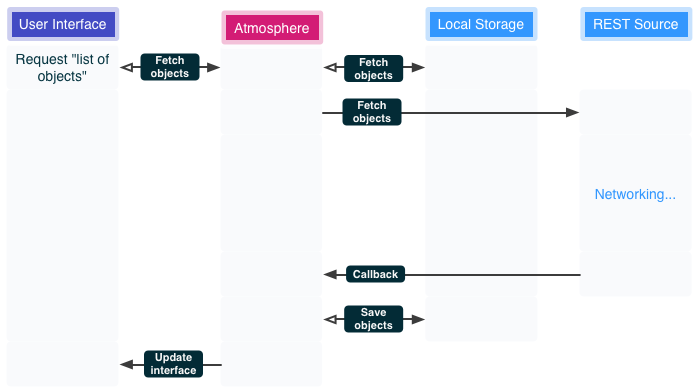
\includegraphics[width=430pt]{LocalStorage1.png}
\caption{Fetching objects using Atmosphere \label{fig:1}}
\end{figure}

The first step to achieve an asynchronous interface is storing some of the application data locally.

Figure \ref{fig:1} presents a situation of fetching a set of objects. When user tries to access a set of objects, \raisebox{-2.5mm}{
\includegraphics[height=0.3in]{Item1.png}} the application will first attempt to retrieve them from local storage, \raisebox{-2.5mm}{
\includegraphics[height=0.3in]{Item2.png}} which is an instant operation. User is provided with some data in zero time.

And the same time the application makes a network request to retrieve the newest data. \raisebox{-2.5mm}{
\includegraphics[height=0.3in]{Item3.png}} When the data is retrieved from the server, \raisebox{-2.5mm}{
\includegraphics[height=0.3in]{Item4.png}} Atmosphere will look at their unique identifiers and try to find an existing copy in the local storage. If the object is found, its attributes are updated and it is saved back to the local storage. If it is not, a new object is created locally. \raisebox{-2.5mm}{
\includegraphics[height=0.3in]{Item5.png}}

The user interface is bound to the local data. When new local data are saved, it is automatically updated to reflect current local data. \raisebox{-2.5mm}{
\includegraphics[height=0.3in]{Item6.png}}

\begin{figure}[ht!]
\centering
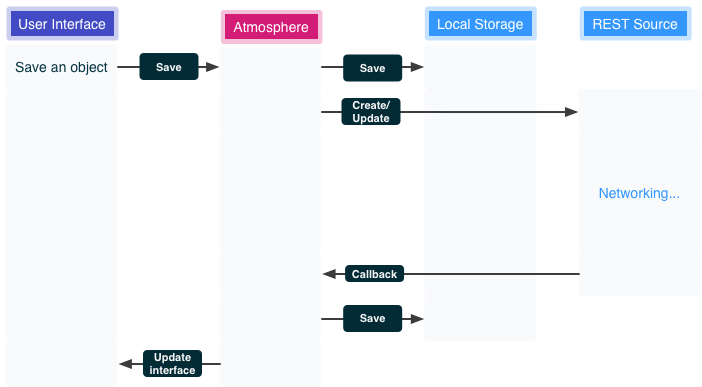
\includegraphics[width=430pt]{LocalStorage2.png}
\caption{Creating objects using Atmosphere \label{fig:2}}
\end{figure}

For making changes the objects, the workflow is similar, depicted in Figure \ref{fig:2}.

When user makes changes to an object, \raisebox{-2.5mm}{
\includegraphics[height=0.3in]{Item1.png}} the changes are immediately written to the local storage. \raisebox{-2.5mm}{
\includegraphics[height=0.3in]{Item2.png}} This operation is instant, so user sees response without any blocking. Now the object is marked as ``changed locally'', which schedules it for synchronization. The synchronization module picks it up, and sends it to the server. \raisebox{-2.5mm}{
\includegraphics[height=0.3in]{Item3.png}} The rest of the process works in the same way as with fetching objects.

Since the REST services have different actions for creating new objects and updating existing ones, it is important to decide whether to send a ``create'' or an ``update'' request. For this purpose Atmosphere keeps track of boolean information which indicates whether the object is ``local only''. This value is set true at the first time object is created, and is changed to false once confirmation about creation is received from the server.

Also, local objects need to be identified somehow. When an object is created locally, it is assigned a temporary identifier in form of UUID. Once it is successfully created remotely, the identifier is updated to permanent identifier assigned by the server.

\subsubsection{Recovering from failure}
\label{sec:failure_recovery}

Synchronization relies on network requests and network connection might be very unreliable at times. Also we have to consider that many of Atmosphere-based applications are developed especially for mobile devices and mobile connection is even less reliable.

The case of fetching objects does not require much attention. If objects fail to load, user will not see them. A notification about network failure can be displayed, but this is responsibility of application logic.

The case of saving object is more complicated. Atmosphere is designed in a way that it will always create a local object first. If the remote request fails, the local object exists, but the remote does not.

This problem is partly solved by keeping track of which objects are ``local only''. (See Figure \ref{fig:recovery1}.) Every object is marked as ``local only'' for as long as its existence was not confirmed by the server. \raisebox{-2.5mm}{
\includegraphics[height=0.3in]{Item1.png}} If one request fails, \raisebox{-2.5mm}{
\includegraphics[height=0.3in]{Item2.png}} the ``local only'' mark remains on object, \raisebox{-2.5mm}{
\includegraphics[height=0.3in]{Item3.png}} and the synchronization is attempted in the next cycle. \raisebox{-2.5mm}{
\includegraphics[height=0.3in]{Item4.png}}

\begin{figure}[htbp]
  \centering
    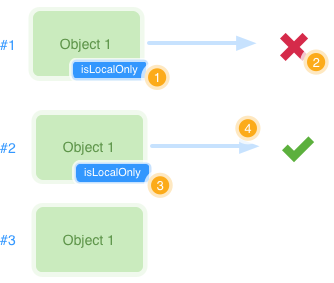
\includegraphics[height=2in]{Recovery1.png}
  \caption{Recovery from failure by keeping track of local objects}
  \label{fig:recovery1}
\end{figure}

A more complicated situation is when the network request is made, processed by the server (therefore the object is created), but the response never makes it back to the client. The object is created remotely, but the client application is not informed about this, so it never removes the ``local only'' mark. Then it tries to create the object again, because the mark was not removed and that results in two objects of the same attributes being created.

A possible solution is assigning permanent ID on the client side. Such solution would expect server to take ID as an argument to the create request.

Now a new object is created on the client side, it is assigned a temporary ID. Then it is sent to the server and server creates object with that ID. The response never comes back to the client, so client makes another create request, with the same ID. Server declines to create another object with the same ID, so it returns a confirmation message for existing object. This time client receives the confirmation message, so the object is marked as not local only.

This solution is not implemented by Atmosphere because it takes server side logic and Atmosphere is purely client-side framework. Implementing such a solution in fact takes only minor modification on server side, and is implemented by Edukit, as described in section \ref{sec:edukit}.

\subsubsection{Exceptions}

Always storing data locally whenever a new object is created might be harmful in certain cases.

For example a web commerce site might provide actions for adding products to the cart, and it might provide an action for submitting the order.

The programmer would probably decide to let Atmosphere manage creation of cart item object. But for order submission, it is better to block user interface, because users want to be sure everything worked. Doing such operation in the background might also lead users into thinking their order was submitted while it was not.

For this purpose, Atmosphere implementations provide a way to create or update an object using a synchronous (in terms of user interface blocking) request. 

\subsubsection{Other solutions}

There are simpler ways of achieving asynchronous interface.

One of them would be to create transient objects that would represent remote objects and still hide networking from the user. Such solution would be less complex because there would have to be no synchronization.

 One drawback would be that opening application for the first time would be slow as user would have to wait for network request to complete. 

Another reason to use local storage and synchronization is that the application can be used offline.

\subsubsection{Notifications}

\begin{figure}[htbp]
  \centering
    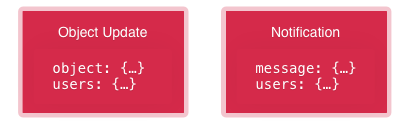
\includegraphics[width=3.5in]{figures/Notifications.png}
  \caption{Types of Atmosphere notifications}
  \label{fig:figures_NotificationServer}
\end{figure}


Atmosphere provides a WebSocket-based notification system for realtime updating of objects. The source application can use this system by making HTTP request to the Atmosphere notification server. (More detailed description is in section \ref{sec:notification_server}.) There are two types of notifications.

The first type is called \textbf{object update}. It is used to propagate an object update to a subset of connected clients. Such message contains object's attributes and list of users to send the notification to. Sending the object update message will cause connected clients to update their local object with the new attributes sent by the server. Using bindings or some other technique, the user interface is updated and user sees the new attributes in real time.

The second type is called \textbf{notification}. A notification contains custom object to be passed to the connected clients. Similarly, it contains list of clients to send the message to. 

A notification message will forward custom object to specified users. The client application is responsible for parsing and processing such message. Atmosphere provides a way for application to subscribe to these notifications.

\subsubsection{Live updates}

Notifications themselves do not suffice in all cases. Take as an example an application where multiple users would like to edit one page together. Once a change is made by one user, a notification could be sent to other users containing the whole page object.

What happens if a page is very long? Sending the whole object would be infeasible. The solution for this problem is to send only the changes made, not the whole objects.

Doing that requires further processing on the server side, to avoid conflicts. This processing can be done using operational transformation. \citep{ot} Since the processing has to happen on the server side, a custom server logic is required. Adding custom server logic is unfortunately not possible for Atmosphere, because one of the design decisions was to support custom REST servers.

This issue could be solved in future by developing a custom extendable Atmosphere server, with support for operational transformation.

\subsection{Components}

\subsubsection{Client}

Client is the computer where Atmosphere-based application is running. It can be a web, desktop or a mobile application.

\begin{figure}[ht!]
\centering
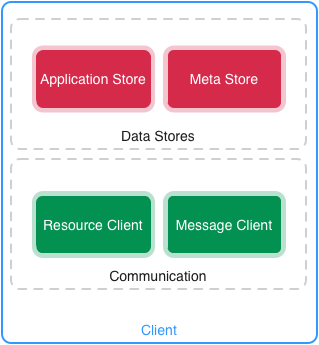
\includegraphics[width=200pt]{MainComponents.png}
\caption{Main components of the client \label{fig:3}}
\end{figure}

The implementations differ across platforms, but from a high level view there are two main component groups: One responsible for storing data locally and one responsible for communication with the HTTP server.

The Application Data Store is a component that is responsible for managing application objects. It is used for tasks like looking up an application object, or updating an application object. This component always depends on native way of storing data. In case of desktop applications, it depends on Core Data framework, etc. 

The Meta Store is a component that is responsible for storing meta objects, objects that encapsulate information that are needed by Atmosphere and that can be ignored by application itself.

List of meta data:

1. ``is object changed'' is a Boolean value that indicates whether the object was changed locally since the last synchronization. 

2. ``is object local only'' is a Boolean value that indicates, whether the object was retrieved from the server, or if it exists only in the local store. 

Components in the communication group are responsible for networking. Resource Client is component responsible for communication with the REST source while Message Client is responsible for communication with the Atmosphere notification server. 

\subsubsection{REST Source}

REST Source is an existing HTTP server. It is not important what language or technology is used to build this server, the only requirement for the server is to implement the basic CRUD methods: create, read, update and delete.

\begin{figure}[ht!]
\centering

\includegraphics[width=250pt]{RestSource.png}
\caption{Communication between the client and the REST source \label{fig:4}}
\end{figure}

The source can be also provided by a third party. For example, in application TaskDo (see section Case Study), the source is RESTful API of Google Tasks. 

Once the server is available and its methods are known, the client must be configured to use the correct methods to create, read, update and delete objects.

The communication between client and the REST source is then performed using HTTP methods.

\subsubsection{Notification server}
\label{sec:notification_server}

\begin{figure}[ht!]
\centering
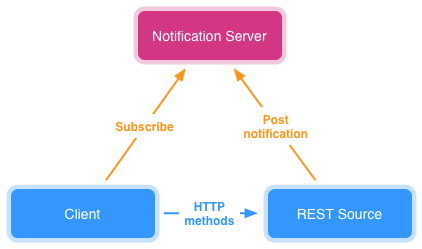
\includegraphics[width=250pt]{NotificationServer.png}
\caption{Use of the notification server by the client and the REST Source \label{fig:5}}
\end{figure}

Notification server is a component that stands between client application and REST source. Client subscribes to notifications on the notification server and the REST source posts notifications to the notification server. 